
\begin{act}\textbf{(Brevet Centres étrangers 10 juin 2024)}\quad
Voici un programme de calcul :
\begin{centered}
	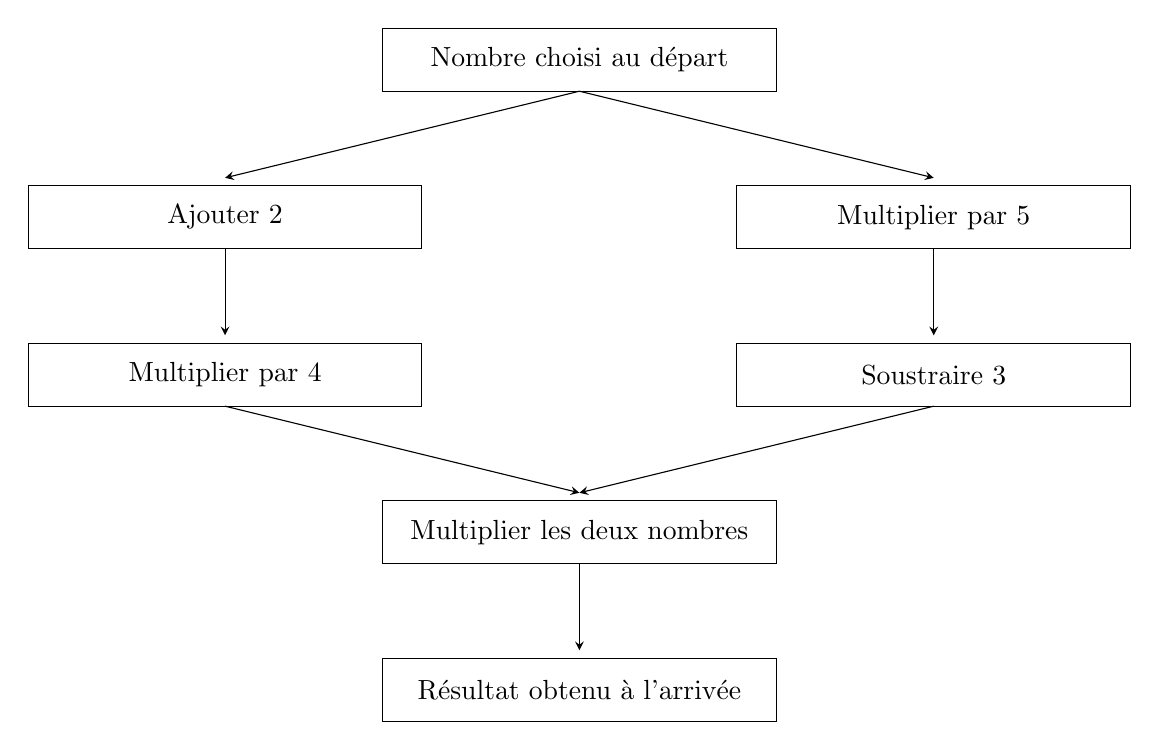
\begin{tikzpicture}[>=stealth]
		\draw[shift={(0,8)}] (-2.5,-0.4) rectangle (2.5,0.4) (0,0) node {Nombre choisi au départ};
		\draw[shift={(-4.5,6)}] (-2.5,-0.4) rectangle (2.5,0.4) (0,0) node {Ajouter 2};
		\draw[shift={(-4.5,4)}] (-2.5,-0.4) rectangle (2.5,0.4) (0,0) node {Multiplier par 4};
		\draw[shift={(4.5,6)}] (-2.5,-0.4) rectangle (2.5,0.4) (0,0) node {Multiplier par 5};
		\draw[shift={(4.5,4)}] (-2.5,-0.4) rectangle (2.5,0.4) (0,0) node {Soustraire 3};
		\draw[shift={(0,2)}] (-2.5,-0.4) rectangle (2.5,0.4) (0,0) node {Multiplier les deux nombres};
		\draw[shift={(0,0)}] (-2.5,-0.4) rectangle (2.5,0.4) (0,0) node {Résultat obtenu à l'arrivée};
		\draw[->] (0,7.6)--(-4.5,6.5);
		\draw[->] (0,7.6)--(4.5,6.5);
		\draw[->] (-4.5,5.6)--(-4.5,4.5);
		\draw[->] (4.5,5.6)--(4.5,4.5);
		\draw[->] (-4.5,3.6)--(0,2.5);
		\draw[->] (4.5,3.6)--(0,2.5);
		\draw[->] (0,1.6)--(0,0.5);
	\end{tikzpicture}
\end{centered}

\begin{enumerate}
	\item Montrer que si on choisit 2 comme nombre de départ, le résultat à l'arrivée est 112 .

	\item Quel est le résultat obtenu à l'arrivée quand on choisit -3 comme nombre de départ?

	\item On choisit $x$ comme nombre de départ.


	Parmi les expressions suivantes, lesquelles permettent d'exprimer le résultat à l'arrivée de ce programme de calcul. Aucune justification n'est demandée.

	\begin{center}
		\begin{tabular}{|c|c|c|c|}
			\hline
			Expression A & Expression B & Expression C & Expression D \\
			\hline
			$(x+2 \times 4)(x \times 5-3)$ & $(4 x+2)(5 x-3)$ & $(4 x+8)(5 x-3)$ & $(x+2) \times 4 \times(5 x-3)$ \\
			\hline
		\end{tabular}
	\end{center}

	\item Trouver les deux nombres de départ qui permettent d'obtenir 0 à l'arrivée. Expliquer la démarche.

	\item Développer et réduire l'expression B.

\end{enumerate}

\end{act}

\begin{act}\textbf{(Brevet Polynésies 27 juin 2024)}\quad
Voici la représentation graphique d'une fonction $f$.


La fonction $f$ est définie par:

\begin{minipage}{0.48\linewidth}
\psset{unit=0.8cm,arrowsize=2pt 3}
\begin{pspicture}(-4,-1)(3.5,3.5)
\psgrid[gridlabels=0pt,subgriddiv=1,gridwidth=0.15pt]
\psaxes[linewidth=1.25pt, labelFontSize=\scriptstyle]{->}(0,0)(-4,-1)(3.5,3.5)
\psplot[plotpoints=600,linewidth=1.25pt,linecolor=red]{-4}{3.5}{x 0.5 mul 1 add}
\end{pspicture}
\end{minipage}

\begin{center}
\renewcommand\arraystretch{1.9}
\begin{tabularx}{\linewidth}{|*{4}{X|}}\hline
$f(x) = 2x - 2$&$f(x) = 2x + 1$&$f(x) = \dfrac x2 - 2$&$f(x) = \dfrac x2 + 1$\\ \hline
\end{tabularx}
\end{center}
\end{act}


\begin{act}\textbf{(Brevet Polynésies 27 juin 2024)}\quad
Dans cet exercice, les deux parties sont indépendantes.

On considère les fonctions $f$ et $g$ définies par 

\begin{center} $f(x) = (x + 2)^2 - x$\quad et \quad  $g(x) = 7x + 4$.\end{center}

\smallskip

\textbf{Partie A}

\medskip

\begin{enumerate}
\item Calculer $f(- 4)$.
\item Déterminer un antécédent de $3$ par la fonction $g$.
\end{enumerate}

\medskip

\textbf{Partie B}

\medskip

Trois élèves, Paul, Jane et Morgane, cherchent à résoudre l'équation $f(x) = g(x)$ par trois méthodes différentes.

\medskip

\begin{enumerate}
\item Paul utilise un tableur.

Il calcule ainsi les images des entiers compris entre $-3$ et $3$ par les fonctions $f$ et $g$.

\begin{center}
\begin{tabularx}{\linewidth}{|l|*{8}{>{\centering \arraybackslash}X|}}\hline
&A &B&C&D&E &F &G &H \\ \hline
1&{\Huge \rput{45}(0,0.5){+}}\vspace{-0.25cm}&$-3$&$ -2$& $-1$& 0 &1 &2 &3\\ \hline
2&$f(x)$&4&2 &2&4&8&14&22\\ \hline
3& $g(x)$& $-17$& $-10$& $-3$& 4& 11& 18& 25\\ \hline
\end{tabularx}
\end{center}

	\begin{enumerate}
		\item Quelle formule a-t-il saisie en cellule B3 puis étirée vers la droite pour compléter la ligne 3 du tableau ?
		\item Avec cette méthode, quelle(s) solution(s) trouve-t-il à l'équation $f(x) = g(x)$ ?
	\end{enumerate}
\item Morgane décide de résoudre cette équation par le calcul.
	\begin{enumerate}
		\item Démontrer que l'équation $f(x) = g(x)$ peut se ramener à l'équation $x^2 - 4x = 0$. 
		\item Factoriser l'expression $x^2 - 4x$.
		\item En déduire les solutions de l'équation $f(x) = g(x)$.
	\end{enumerate}
\end{enumerate}
\end{act}


\begin{act}\textbf{(Brevet Amérique du Nord 29 mai 2024)}\quad
Un cinéma propose trois tarifs :

\textbf{Tarif \og{} Classique \fg{} :} La personne paye chaque entrée 11\euro{}.

	\textbf{Tarif \og{} Essentiel \fg{} :} La personne paye un abonnement annuel de 50 \euro{} puis chaque entrée coûte 5 \euro{}.

\textbf{Tarif \og{} Liberté \fg{} :} La personne paye un abonnement annuel de 240 \euro{} avec un nombre d'entrées illimité.

\begin{enumerate}
	\item Avec le tarif \og{} Classique \fg{}, une personne souhaite acheter trois entrées au cinéma.

	Combien va-t-elle payer ?

	\item Avec le tarif \og{} Essentiel \fg{}, une personne souhaite aller huit fois au cinéma.

	Montrer qu'elle va payer 90 \euro{}.

	\item Dans la suite, $x$ désigne le nombre d'entrées au cinéma.

	On considère les trois fonctions $f, g$ et $h$ suivantes :

	\hfill~$f: x \longmapsto 50+5 x \qquad g: x \longmapsto 240 \qquad h: x \longmapsto 11 x$\hfill~

	Associer, sans justifier, chacune de ces fonctions au tarif correspondant.
\end{enumerate}

Le graphique ci-dessous représente le prix à payer en fonction du nombre d'entrées pour chacun de ces trois tarifs.

\begin{center}
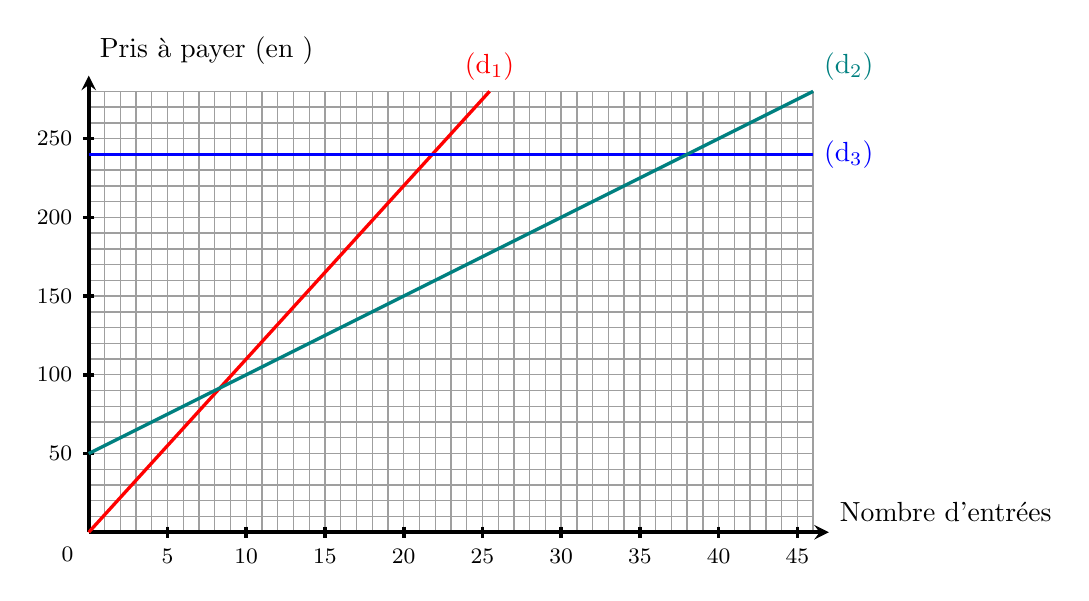
\begin{tikzpicture}[x=2mm,y=0.2mm,>=stealth]
		\draw [color = gray!75, line width = 0.5pt, xstep=1, ystep = 10] (0,0) grid (46,280);
	\draw[->,line width = 1.3pt] (0,0) -- (47,0) node[above right]{Nombre d'entrées};
	\foreach \x in {5,10,...,45}
	\draw[shift={(\x,0)},color=black,line width = 1.3pt] (0pt,2pt) -- (0pt,-2pt) node[below, fill = white] {\footnotesize $\np{\x}$};
	\draw[->,line width = 1.3pt] (0,0) -- (0,290) node[above right]{Pris à payer (en \euro{})};
	\foreach \y in {50,100,...,250}
	\draw[shift={(0,\y)},color=black,line width = 1.3pt] (2pt,0pt) -- (-2pt,0pt) node[left, fill = white] {\footnotesize $\np{\y}$};
	\draw[color=black] (-2pt,-2pt) node[below left] {{\footnotesize 0}};
	\draw[line width=1.2pt,color=red](0,0)--(25.4545,280) node[above]{$(\mathrm{d}_1)$};
	\draw[line width=1.2pt,color=blue](0,240)--(46,240) node[right]{$(\mathrm{d}_3)$};
	\draw[line width=1.2pt,color=teal](0,50)--(46,280) node[above right]{$(\mathrm{d}_2)$};
\end{tikzpicture}
\end{center}

La droite $(\mathrm{d}_{1})$ représente la fonction correspondant au tarif \og{} Classique \fg{}.

La droite $(\mathrm{d}_{2})$ représente la fonction correspondant au tarif \og{} Essentiel \fg{}.

La droite $(\mathrm{d}_{3})$ représente la fonction correspondant au tarif \og{} Liberté \fg{}.

\begin{enumerate}[resume]

	\item Quel tarif propose un prix proportionnel au nombre d'entrées ?

	\item Pour les questions suivantes, aucune justification n'est attendue.

	\begin{enumerate}
		\item Avec 150 \euro{}, combien peut-on acheter d'entrées au maximum avec le tarif \og{} Essentiel \fg{}?
		\item À partir de combien d'entrées, le tarif \og{} Liberté \fg{} devient-il le tarif le plus intéressant?
		\item Si on décide de ne pas dépasser un budget de 200 \euro{}, quel est le tarif qui permet d'acheter le plus grand nombre d'entrées ?
	\end{enumerate}
\end{enumerate}
\end{act}

\begin{act}\textbf{(Brevet Asie 18 juin 2024)}\quad
Une forme factorisée de l'expression littérale $4x^2 - 9$ est\ldots \index{identité remarquable}

\begin{center}
\begin{tabularx}{\linewidth}{|*{4}{>{\centering \arraybackslash}X|}}\hline
Réponse A &Réponse B &Réponse C &Réponse D\\ \hline
$(4x- 3)(4x +3)$ &$(2x- 3)(2x +3)$& $(2x- 3)^2$& $(4x- 9)(4x +9)$\\ \hline
\end{tabularx}
\end{center}
\end{act}

\begin{act}
Des amis habitent Strasbourg et préparent leurs vacances.

Cette année ils ont décidé de partir découvrir une grande ville française pendant une semaine. 

Pour s'y rendre, ils louent une voiture. Une fois arrivés sur place, ils feront ensuite tous leurs trajets à pied ou en transport en commun.

Une agence de location de voitures propose les trois formules suivantes pour une location sur une semaine :

\begin{center}
\begin{tabularx}{\linewidth}{*{3}{>{\centering \arraybackslash}X}}\hline
Formule A&Formule B&Formule C\\ \hline
0,50~\euro{} pour chaque kilomètre parcouru&
 Forfait fixe de 300~\euro{}
puis 0,25~\euro{} pour chaque kilomètre parcouru&
Forfait fixe de 900~\euro{} pour un kilométrage illimité.\\ \hline
\end{tabularx}

\bigskip

\textbf{Tableau indicatif des distances (en km) entre des villes françaises}
\medskip

\begin{tabularx}{\linewidth}{*{7}{>{\centering \arraybackslash}X}}
Bordeaux&&&&&&\\ \cline{1-1}
675& Grenoble&&&&&\\ \cline{1-2}
792& 771& Lille&&&&\\ \cline{1-3}
 555 &280&1005&Marseille&&&\\ \cline{1-4}
338 &741&584& 909& Nantes&&\\ \cline{1-5}
546& 585&215 &772& 379& Paris&\\ \cline{1-6}
907 &506& 498 &803& 864& 442&Strasbourg\\ \cline{1-7}
\end{tabularx}
\end{center}

Exemple: la distance la plus courte entre Nantes et Grenoble est de 741 km.

\medskip

\textbf{PARTIE A} : Les amis souhaitent se rendre à Marseille. Ils ont un budget de \np{1000} \euro{} pour le voyage.

\medskip

\begin{enumerate}
\item Quelle distance, en km, vont-ils parcourir pour le trajet aller-retour ?
\item En choisissant la formule B, montrer que la location de voiture coûtera $701,50$~\euro.
\item Quelle est la formule la plus avantageuse ?
\item Voici des informations pour le voyage :

\begin{center}
\begin{tabularx}{\linewidth}{|*{3}{>{\centering \arraybackslash}X|}}\hline
Information 1&Information 2&Information 3\\ \hline
\small Prix moyen du gazole en 2023 &\small Voiture proposée&\small  Coût total pour les péages\\
\small 1,87~\euro{} par litre&\small Type de carburant: gazole. Consommation: 5,6~L pour 100 km&\small  115,80~\euro \\ \hline
\end{tabularx}
\end{center}

Leur budget sera-t-il suffisant ?

\emph{Dans cette question, toute trace de recherche sera prise en compte dans la correction}.
\end{enumerate}
\medskip

\medskip

\textbf{PARTIE B }: Étude des formules 

\begin{center}
\begin{tabularx}{\linewidth}{|*{3}{>{\centering \arraybackslash}X|}}\hline
Formule A&Formule B&Formule C\\ \hline
0,50~\euro{} pour chaque kilomètre parcouru&Forfait fixe de 300~\euro{}
puis 0,25~\euro{} pour chaque kilomètre parcouru&Forfait fixe de $900$~\euro{} pour un kilométrage illimité.\\ \hline
\end{tabularx}
\end{center}

\begin{enumerate}[resume]
\item Soit $x$ le nombre de kilomètres parcourus, exprimer en fonction de $x$ le prix payé pour chaque formule de location.
\item On a représenté ci-dessous, pour chacune des formules, le coût de la location (en euros) en fonction de la distance parcourue (en kilomètres).\index{fonction affine}

Associer chaque courbe à la formule de location correspondante. \emph{Ne pas justifier}.\index{lecture graphique}

\begin{center}
\psset{xunit=0.004cm,yunit=0.0075cm,arrowsize=2pt 3,labels=none}
\begin{pspicture}(-200,-50)(2600,1300)
\uput[r](0,1250){Coût de la location (en \euro)}
\uput[d](1800,0){Distance parcourue (en km)}
\psaxes[linewidth=1.25pt,labels=none,Dx=200,Dy=200]{->}(0,0)(0,0)(2600,1300)
\psaxes[linewidth=1.25pt,labels=none,Dx=200,Dy=200](0,0)(0,0)(2600,1300)
\psline[linewidth=1.25pt,linecolor=blue](2600,1300)\rput{45}(300,120){\blue Courbe 3}
\psline[linewidth=1.25pt,linecolor=red](0,300)(2600,950)\rput{25}(400,380){\red Courbe 2}
\psline[linewidth=1.25pt,linecolor=cyan](0,900)(2600,900)\uput[u](400,900){\cyan Courbe 1}
\uput[d](200,0){200}\uput[l](0,200){200}
\end{pspicture}
\end{center}

\item Résoudre l'équation 
\[0,25x + 300 = 0,5x.\]\index{résolution d'équation}
 Interpréter ce résultat.
\item 
	\begin{enumerate}
		\item Si la distance parcourue est de \np{2500}~km, quelle formule doit-on choisir pour payer le moins cher ? Ne pas justifier.
		\item Donner une distance parcourue pour laquelle la formule A est la plus intéressante. Ne pas justifier.
		\item Déterminer graphiquement quelle formule de location est la moins chère en fonction de la distance parcourue pour une distance inférieure à \np{2600}~km.\index{lecture graphique}
	\end{enumerate}
\end{enumerate}
\end{act}

\begin{act}\textbf{()}
Pour se promener le long d'un canal, deux sociétés proposent une location de bateaux électriques.

Les bateaux se louent pour un nombre entier d'heures.

\medskip

\begin{enumerate}
\item \textbf{Étude du tarif proposé par la société A}

\medskip

Pour la société A, le prix à payer pour la location d'un bateau en fonction de la durée de location en heure est donné par le graphique suivant :

\begin{centered}
\psset{xunit=1.4cm,yunit=0.028cm,arrowsize=2pt 3}
\begin{pspicture}(-0.5,-20)(8.25,295)
\multido{\n=0.0+0.5}{17}{\psline[linewidth=0.6pt](\n,0)(\n,280)}
\multido{\n=0+10}{29}{\psline[linewidth=0.6pt](0,\n)(8.25,\n)}
\psaxes[linewidth=1.25pt,Dy=50]{->}(0,0)(0,0)(8.25,280)
\psplot[linewidth=1.25pt,linecolor=blue,plotpoints=500]{0}{8.25}{30 x mul}
\uput[d](6.5,-15){Durée de location (en heures)}
\uput[r](0,290){Prix payé (en \euro)}
\rput{31}(8,250){Société A}
\end{pspicture}
\end{centered}

Répondre aux questions ci-dessous à l'aide du graphique.

Aucune justification n'est attendue pour les questions a. et b.
	\begin{enumerate}
		\item Quel prix va-t-on payer en louant un bateau pour 2 heures ?
		\item On dispose d'un budget de $100$~\euro, combien d'heures entières peut-on louer un bateau ?
		\item Expliquer pourquoi le prix est proportionnel à la durée de location.
		\item En déduire à l'aide d'un calcul, le prix à payer pour une durée de location de $10$~heures.
	\end{enumerate}
\item \textbf{Étude du tarif proposé par la société B}

\medskip

La société B propose le tarif suivant : $60$~\euro{} de frais de dossier plus $15$~\euro{} par heure de location.
	\begin{enumerate}
		\item Montrer qu'en louant un bateau pour une durée de 2 heures, le prix à payer sera de $90$~\euro.
		\item On désigne par $x$ le nombre d'heures de location. On appelle $f$ la fonction qui, au nombre d'heures de location, associe le prix, en euro, avec le tarif proposé par la société B.

On admet que $f$ est définie par : $f(x) = 15x + 60$.

Sur le graphique donné en ANNEXE à rendre avec la copie, tracer la courbe représentative de la fonction $f$.
		\item Le prix payé est-il proportionnel à la durée de location ?
	\end{enumerate}
\item \textbf{Comparaison des deux tarifs}
	\begin{enumerate}
		\item On souhaite louer un bateau pour une durée de 3 heures.

Quelle société doit-on choisir pour avoir le tarif le moins cher ?

Quel prix va-t-on payer dans ce cas ?
		\item Pour quelle durée de location le prix payé est-il identique pour les deux sociétés ?
	\end{enumerate}
\end{enumerate}
\end{act}


\begin{act}\textbf{(Brevet Métropole Antilles-Guyane 26 juin 2023)}
Voici deux programmes de calcul.

\begin{center}
	\begin{tabularx}{\linewidth}{|X|X|}\hline
Programme A &Programme B\\
$\bullet~~$ Choisir un nombre				&$\bullet~~$ Choisir un nombre\\
$\bullet~~$ Multiplier ce nombre par $-2$	&$\bullet~~$ Soustraire 5 à ce nombre\\
$\bullet~~$Ajouter 5 à ce résultat.			&$\bullet~~$ Multiplier le résultat par 3\\
											&$\bullet~~$ Ajouter 11 au résultat\\ \hline
	\end{tabularx}
\end{center}

\begin{enumerate}
	\item
	\begin{enumerate}
		\item Montrer que, si on choisit $- 3$ comme nombre de départ, le résultat obtenu avec le programme A est 11.
		\item Quel résultat obtient-on avec le programme B si on choisit 5,5 comme nombre de départ ?
	\end{enumerate}
	\item En désignant par $x$ le nombre de départ, on obtient $- 2x + 5$ comme résultat avec le programme A.

	Montrer, qu'avec le même nombre de départ, le résultat du programme B est égal à $3x - 4$.
\end{enumerate}
\begin{minipage}{0.56\linewidth}
	\begin{enumerate}[resume]
		\item
		\begin{enumerate}
			\item On a représenté ci-contre les fonctions $f$ et $g$ définies par $f(x) = -2x + 5$
			et $g(x) = 3x - 4$.

			Associer, en justifiant, chaque droite à la fonction qui lui correspond.
			\item Par lecture graphique, donner, le plus précisément possible, le nombre dont l'image est la même par la fonction $f$ et la fonction $g$.
		\end{enumerate}
	\end{enumerate}
\end{minipage}\hfill
\begin{minipage}{0.42\linewidth}
	\psset{xunit=1cm,yunit=0.7cm,arrowsize=2pt 3}
	\begin{pspicture*}(-1.02,-4)(5,7.02)
		\psgrid[gridlabels=0pt,subgriddiv=1,gridwidth=0.3pt]
		\psaxes[linewidth=1.25pt,labelFontSize=\scriptstyle]{->}(0,0)(-1,-4)(5,7)
		\psplot[plotpoints=500,linewidth=1.25pt]{-1}{5}{x 3 mul 4 sub}\uput[dr](3.4,6){$(D_1)$}
		\psplot[plotpoints=500,linewidth=1.25pt]{-1}{5}{5 x 2 mul sub}\uput[ur](4.3,-4){$(D_2)$}
	\end{pspicture*}
\end{minipage}

\medskip

\begin{enumerate}[start=4]
	\item Déterminer par le calcul le nombre de départ pour lequel les programmes A et B donnent le même résultat.
\end{enumerate}
\end{act}


\begin{act}\textbf{(Brevet Métropole Antilles-Guyane 18 septembre 2023)}
Quelle est la valeur de l’expression 

$x^2 + 3x - 5$ pour $x  =  - 2$ ?%& $- 15$&5&$- 7$
\end{act}

\begin{act}\textbf{(Brevet Métropole Antilles-Guyane 18 septembre 2023)}
Une piscine propose deux tarifs d'entrée pour l'année 2023.

\textbf{Tarif A} : $5,90$~\euro{} l'entrée.

\textbf{Tarif B} : $4,40$~\euro{} l'entrée avec une carte d'abonnement de $30$~\euro{} valable toute l'année.

\medskip

\begin{enumerate}
\item 
	\begin{enumerate}
		\item Quel est le prix total pour $10$ entrées avec le tarif A ? 
		\item Quel est le prix total pour $10$ entrées avec le tarif B ?
	\end{enumerate}
\item  On note $f$ et $g$ les fonctions qui modélisent les prix, en euro, respectivement du tarif A et du tarif B en fonction du nombre $x$ d'entrées.

Donner l'expression de $f(x)$, puis celle de $g(x)$.
\item 
	\begin{enumerate}
		\item Résoudre l'équation $5,90x = 4,40x + 30$.
		\item Quel est le nombre d'entrées pour lequel les tarifs A et B donnent le même prix à payer ?
	\end{enumerate}
\end{enumerate}

On relève le nombre d'entrées par mois durant une année.

\begin{center}
\begin{tabularx}{\linewidth}{|m{1.5cm}|*{12}{>{\centering \arraybackslash \footnotesize}X|}}\hline
\footnotesize Mois	&Jan.	& Fév.& Mars& Avril& Mai& Juin& Juillet& Août& Sept.& Oct.& Nov.& Déc.\\ \hline
\footnotesize 
Nombre d'entrées	&\np{12500} &\np{13700} &\np{10400} &\np{13600} &\np{12300} &\np{11700} &\np{10400} &\np{11600} &\np{10200} &\np{13800} &\np{12600} &\np{11800}\\ \hline
\end{tabularx}
\end{center}
\begin{enumerate}[resume]
\item
	\begin{enumerate}
		\item Calculer le nombre moyen d'entrées par mois.
		\item Calculer l'étendue du nombre d'entrées par mois.
	\end{enumerate}
\item La piscine a la forme d'un pavé droit de longueur $50$~m, de largeur $25$~m et de profondeur $3$~m. En admettant qu'elle soit entièrement remplie, déterminer en m$^3$, le volume d'eau qui sera évacué pour réaliser la vidange.
\end{enumerate}
\end{act}


\begin{act}\textbf{(Brevet Nouvelle-Calédonie 7 décembre 2023)}
\begin{enumerate}
\item 
	\begin{enumerate}
		\item La fonction $f$, dont la représentation graphique est ci-dessous  est-elle une fonction affine ? Justifier votre réponse.
		
		\begin{centered}
\psset{unit=0.75cm,arrowsize=2pt 3}
\begin{pspicture*}(-5,-5.1)(6,13)
\psgrid[gridlabels=0pt,subgriddiv=1,gridwidth=0.4pt]
\psaxes[linewidth=1.25pt,labelFontSize=\scriptstyle]{->}(0,0)(-5,-5)(6,13)
\psplot[plotpoints=2000,linewidth=1.25pt,linecolor=red]{-5}{5}{x 1 sub x 3 add mul}
\uput[d](5.75,0){$x$}\uput[l](0,12.75){$y$}\uput[r](2.95,11.15){\red $\mathcal{C}_f$}
\end{pspicture*}
\end{centered}

		\item À l'aide de ce graphique, compléter ce tableau de valeurs de la fonction $f$ :
		\begin{centered}
\begin{tabularx}{\linewidth}{|*{8}{>{\centering \arraybackslash}X|}}\hline
	&A		&B		&C		&D		&E		&F		&G\\ \hline
1	&$x$	&$-3$	&$-2$	&$-1$	&0		&1		&2\\ \hline
2	& $f(x)$& 0 	& $-3$	&\ldots	&\ldots	&\ldots	&\ldots\\ \hline
\end{tabularx}
\end{centered}

	\end{enumerate}

Parmi les trois formules suivantes, l'une correspond à l'expression de la fonction $f$.

Elle a été saisie dans la cellule B2 puis étendue dans la cellule C2 du tableau de l'annexe.

\begin{center}
\begin{tabularx}{\linewidth}{|*{3}{>{\centering \arraybackslash}X|}}\hline
=B1 + 3 &=(B1 + 3)$*$(B1 $-$ 1)& =SOMME(B1 : G1) \\ \hline
\end{tabularx}
\end{center}
\begin{enumerate}[resume] 
		\item Noter la bonne formule sur votre copie.
	\end{enumerate}
\item On considère la fonction affine $g$ définie par $g(x) = 2x + 1$. 
	\begin{enumerate}
		\item Calculer l'image de $-2$ par la fonction $g$.
		\item Calculer $g(3)$.
		\item Déterminer l'antécédent de $2$ par la fonction $g$.
		\item Tracer, sur le graphique de l'annexe, la représentation graphique de la fonction~$g$.
	\end{enumerate}
\item L'expression de la fonction $f$ ci-dessus est $f(x) = (x + 3)(x - 1)$.
	\begin{enumerate}
		\item Développer et réduire l'expression $(x + 3)(x - 1)$.
		\item Pour quelle(s) valeur(s) de $x$, a-t-on $f(x) = g(x)$ ?
	\end{enumerate}
\end{enumerate}
\end{act}